\documentclass[aspectratio=169]{beamer}
\usepackage[utf8]{inputenc} % codificacao de caracteres
\usepackage[T1]{fontenc}    % codificacao de fontes
\usepackage[english]{babel}  % idioma
\usepackage{graphics,amssymb,amsfonts,amsmath,xfrac}
\usepackage{tikz}
\usepackage{enumerate,hyperref}
\usepackage{palatino}	% Fonte sem serifa
\usepackage{ragged2e}	% Paragrafo justificado
%\usepackage{minted}	% Highlight para codigos de programacao
\usepackage{booktabs} % tabelas
\usepackage{multicol}
\usepackage{multirow}
%\usepackage[table]{xcolor}


% Veja mais temas e cores em http://www.hartwork.org/beamer-theme-matrix/
\usetheme{Montpellier}         % tema
\usecolortheme{orchid}      % cores
\usefonttheme[onlymath]{serif} % fonte modo matematico
% Colocando numero de paginas no slide
\setbeamertemplate{footline}[frame number]



\DeclareGraphicsExtensions{.pdf,.jpg,.png} % compilamos apenas com pdflatex
\graphicspath{{figuras/}} % caminho onde as figuras estarao disponiveis




% ---------------------------------------------------------------------------- %
% T�tulo                                                                       %
% ---------------------------------------------------------------------------- %

\title[\sc{Teoria de Circuitos Eletrônicos 1}]{\LARGE Aula 9 - Exercise Class 3}
\author[Prof. Marcelino Andrade]{Prof. Marcelino Andrade}
\institute{Faculdade UnB Gama} % opcional
\date{\today}

\begin{document}
\justifying % Paragrafo justificado
\pagebreak
\small
\begin{frame}
  \titlepage
\end{frame}


% ----------------- NOVO SLIDE --------------------------------
\begin{frame}{Contents\newline}

\tableofcontents
\begin{center}	
     		Introduction to Electric Circuits by James A. Svoboda, Richard C. Dorf, 9th Edition			
\end{center}	
\end{frame}

% ----------------- NOVA SECÇÂO -----------------------------
\section{CHAPTER 3 Resistive Circuits}
% ----------------- NOVO SLIDE --------------------------------
\begin{frame}[fragile]
	\frametitle{Resistive Circuits}
\begin{tabular}{ll}
	\begin{columns}
		\begin{column}{1\textwidth}  %%<--- here
		\textbf{Problem 3.6-11} - Find $i$ and $R_{eq\ a-b}$ if $v_{ab}=40$ V in the circuit of Figure below.\\
		\begin{center}
    			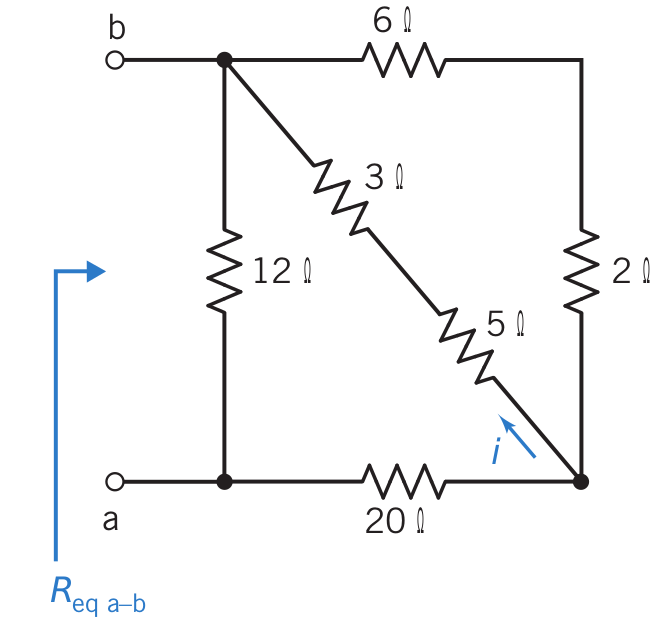
\includegraphics[height=3.6cm]{figure1.png}	
		\end{center}	
		\scalebox{0.8}{Answer: $i=\frac{5}{6}A$ and  $R_{eq\ a-b}=8 \Omega$.}
		\end{column}
	\end{columns}
\end{tabular}
\end{frame}

% ----------------- NOVA SECÇÂO -----------------------------
\section{CHAPTER 4 Methods of Analysis of Resistive Circuits}
% ----------------- NOVO SLIDE --------------------------------
\begin{frame}[fragile]
	\frametitle{Methods of Analysis of Resistive Circuits}
\begin{tabular}{ll}
	\begin{columns}
		\begin{column}{1\textwidth}  %%<--- here
		\textbf{Problem 4.4-2} - Find $i_b$ for the circuit shown in Figure below.\\
		\begin{center}
    			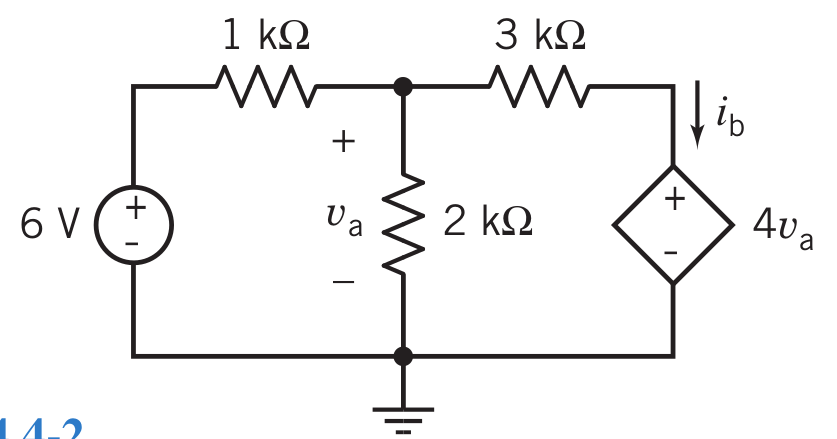
\includegraphics[height=3.6cm]{figure2.png}	
		\end{center}	
		\scalebox{0.8}{Answer: $i_b= -12mA$.}
		\end{column}
	\end{columns}
\end{tabular}
\end{frame}

% ----------------- NOVA SECÇÂO -----------------------------
\section{CHAPTER 5 Circuit Theorems}
% ----------------- NOVO SLIDE --------------------------------
\begin{frame}[fragile]
	\frametitle{Circuit Theorems}
\begin{tabular}{ll}
	\begin{columns}
		\begin{column}{1\textwidth}  %%<--- here
		\textbf{Problem 5.4-4} -Find the Thevenin equivalent circuit for the circuit shown in Figure below.\\
		\begin{center}
    			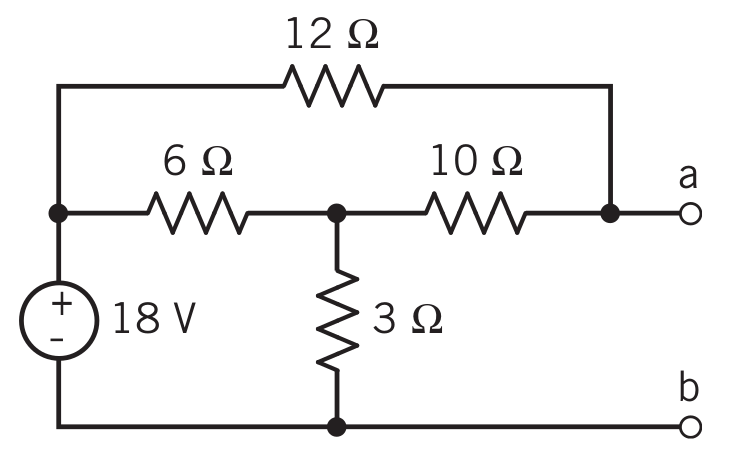
\includegraphics[height=3.6cm]{figure3.png}	
		\end{center}	
		\scalebox{0.8}{Answer: $v_{t}= 12V \ and \ R_{t}=6\Omega$}
		\end{column}
	\end{columns}
\end{tabular}
\end{frame}

% ----------------- NOVA SECÇÂO -----------------------------
\section{CHAPTER 6 The Operational Amplifier}
% ----------------- NOVO SLIDE --------------------------------
\begin{frame}[fragile]
	\frametitle{Operational Amplifier}
\begin{tabular}{ll}
	\begin{columns}
		\begin{column}{1\textwidth}  %%<--- here
		\textbf{Problem 6.4-161} - The circuit shown in Figure below has one input,
$v_s$ , and one output, $v_o$. Express the gain $\frac{v_o}{v_s}$ in terms of the
resistances $R_1$ , $R_2$ , $R_3$ , $R_4$ , and $R_5$. Design the circuit so that
$v_o=-20 v_s$.\\
		\begin{center}
    			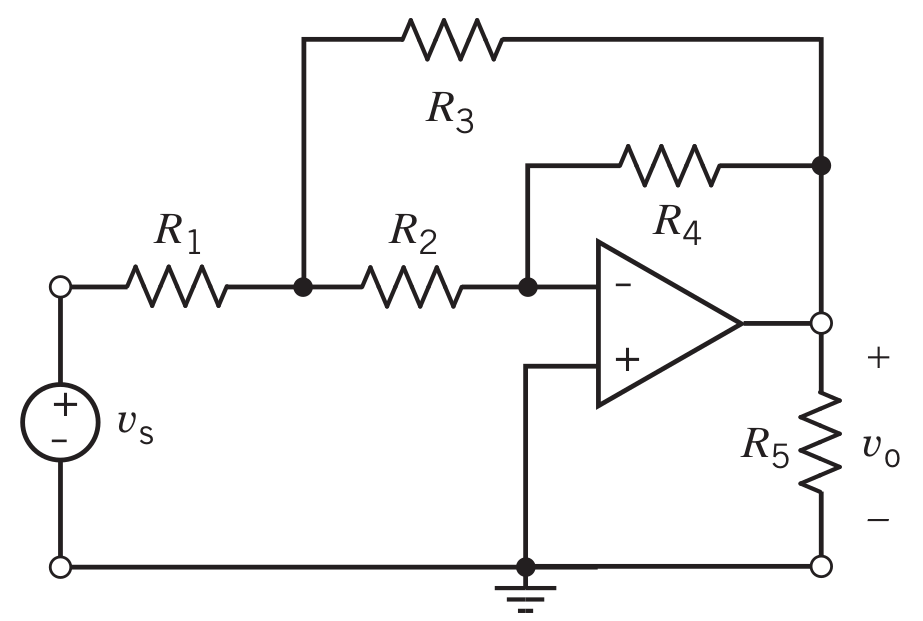
\includegraphics[height=2.6cm]{figure4.png}	
		\end{center}	
		\scalebox{0.8}{Answer: $\frac{v_o}{v_s}= \frac{-R_3R_4}{R_1R_2+R_1R_3+R_2R_3+R_1R_4}$ and $R_1=1\Omega$, $R_2=78\Omega$, $R_3=100\Omega$ e $R_4=2000\Omega$}
		\end{column}
	\end{columns}
\end{tabular}
\end{frame}
%----------------- NOVA SECÇÂO -----------------------------
\section{CHAPTER 7 Energy Storage Elements}
% ----------------- NOVO SLIDE --------------------------------
\begin{frame}[fragile]
	\frametitle{Energy Storage Elements}
\begin{tabular}{ll}

\begin{columns}
  \begin{column}{1\textwidth}
\textbf{Problem 7.8-6} - The switch in the circuit shown in Figure below
has been open for a long time before it closes at time
$t = 0$. Determine the values of $v_L(0^-)$, the voltage across the
inductor immediately before the switch closes, and $v_L(0^+)$,
the voltage across the inductor immediately after the switch
closes.\\
  \end{column}
\end{columns}\\

	\begin{columns}
		\begin{column}{1\textwidth}  %%<--- here
		\begin{center}
    			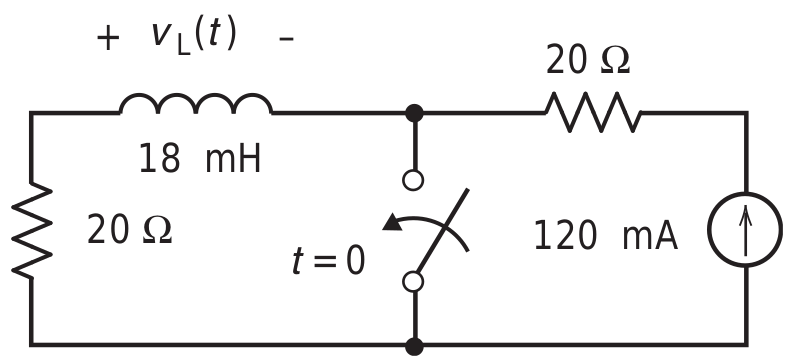
\includegraphics[height=2.6cm]{figure5.png}
		\end{center}	
\scalebox{0.8}{Answer: $v_L(0^-)=0V$ and $v_L(0^+)=2.4V$}
		\end{column}

		
		
		
		
	\end{columns}
\end{tabular}
\end{frame}
% ----------------- NOVA SECÇÂO -----------------------------

\end{document} 






